\chapter{Authenticated Encryption with Associated Data}\label{chap:aead}
Sappiamo che un cifratore ben strutturato può garantire \textit{confidentiality}, ovvero abbiamo semantic security contro attacchi \textit{CPA}. Tuttavia, per garantire \textit{integrity} abbiamo fatto fino ad ora un discorso separato, basato su un codice generato tramite una funzione hash.
\begin{remark}
Se un attaccante dovesse essere \textit{"attivo"}, ovvero in grado di creare un testo cifrato il cui MAC sia valido, non avremmo modo di garantire \textit{integrity}.
\end{remark}
\begin{definition}[Chosen Ciphertext Attack]\label{def:cca}
Scenario di attacco nel quale un hacker può fare, oltre all'eavesdropping, anche una cifratura di un plaintext di sua creazione che è in grado di modificare un messaggio.\\
\textbf{Rompendo}, di fatto, \textbf{sia confidentiality che integrity}.
\end{definition}
Vediamo due esempi di come \textbf{rompere confidentiality} porti ad una \textbf{rottura di integrity}.
\begin{example}Consideriamo l'invio di un pacchetto \textit{TCP/IP} da \textit{\textbf{A}} verso \textit{\textbf{B}} passando per un web-server che gestisce lo stack TCP/IP. Facciamo le seguenti supposizioni: 
\begin{enumerate}
    \item Il pacchetto attraversa un server sul quale \textit{\textbf{E}} può intercettare i processi su una porta specifica. Per semplicità il \textbf{pacchetto} sia \textbf{diretto} sulla \textbf{porta 80 di B}, mentre \textbf{E} può \textbf{leggere} dalla \textbf{porta 25}. 
    \item Il canale di trasferimento è \textbf{protetto} con \textbf{sola encryption} (garantiamo solo \textit{confidentiality}).
    \item L'attaccante è in grado di generare un cipher-text il cui contenuto cambia la porta da 80 a 25. 
\end{enumerate}
Poiché non ci stiamo preoccupando di integrity (e quindi non usiamo un MAC), \textit{\textbf{E}} può leggere i dati in chiaro dal server dalla porta 25. In particolare, se viene usato \textbf{AES-CBC} è semplice in quanto basta fare uno xor. Vediamo lo schema:
\end{example}
\begin{figure}[h]
    \centering
    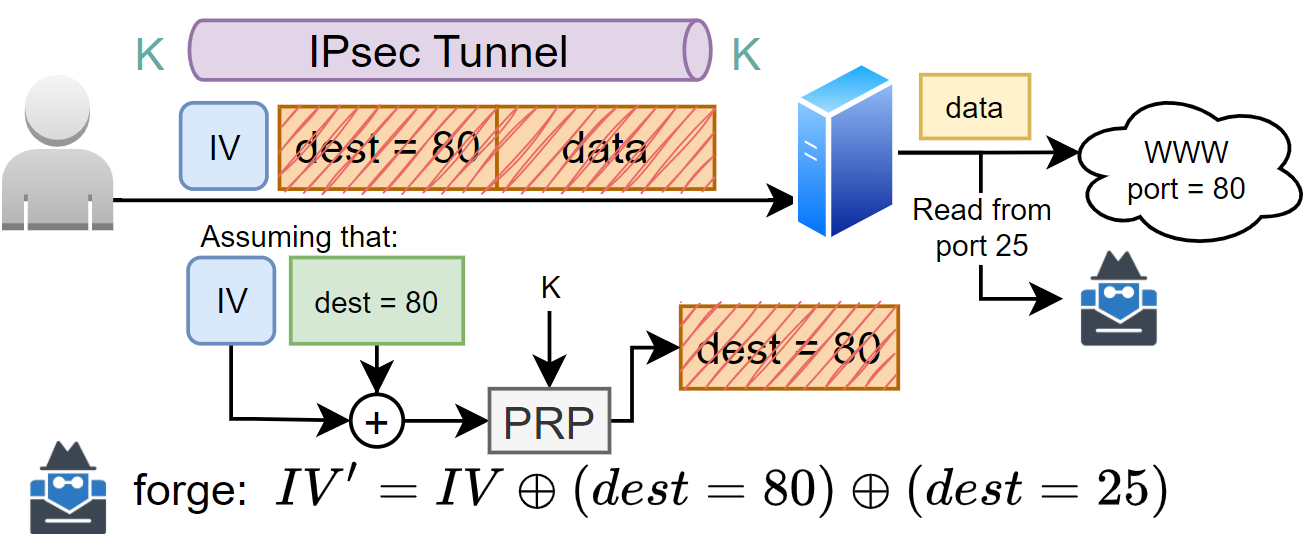
\includegraphics[width=\linewidth]{image/portredirect.png}
    \caption{Broken Confidentiality}
    \label{fig:portredirect}
\end{figure}
Inserendo l'\textit{IV'}, nel processo di cifratura possiamo cambiare la porta. Infatti:
\begin{figure}[h]
    \centering
    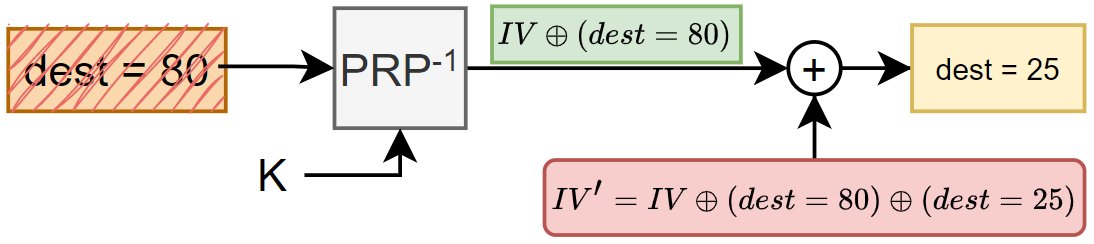
\includegraphics[width=\linewidth]{image/portredirectdec.png}
    \caption{Decription}
    \label{fig:decriptionport}
\end{figure}
\begin{example}[ ACK-Oracle:]Supponiamo che A stia usando una \textit{remote terminal app}, dove ogni keystroke viene cifrato in CTR e inviato verso un server. I \textit{"poteri"} di E sono i seguenti:
\begin{enumerate}
    \item \textbf{E non ha accesso al backend}.
    \item La cifratura viene fatta in CTR mode.
    \item L'header è tipicamente noto poiché la struttura è definita da standard e i valori possono essere predetti.
    \item E può copiare il messaggio cifrato di A.
    \item [\textcolor{red}{FACT}:]Lo stack TCP/IP processa solo pacchetti validi, rispondendo con un \textit{ACK} solo ai pacchetti con checksum valido. Il checksum è calcolato in funzione dell'header del pacchetto e del carattere inviato D.
\end{enumerate}
\begin{remark}
Il protocollo restituisce pertanto \textbf{DUE} risultati, indicandoci quali sono i pacchetti corretti e non rispondendo nulla se il pacchetto non lo è.
\end{remark}
Supponiamo di fare molte copie del messaggio e di provare $\forall{t,s}$ ad inviare verso il server una copia modificata nel campo checksum e carattere calcolando $checksum\oplus{t}$ e $D\oplus{s}$. Per ogni volta in cui il server dello stack TCP/IP risponderà con un ACK, otteniamo un'equazione valida del tipo:
\[checksum(pkt-hdr,D\oplus{s})=t\oplus{cheksum(pkt-hdr, D)}\]
Poiché l'header del pacchetto è noto (punto 3), mentre la coppia {checksum, D} non lo è, il sistema è risolubile. Una volta trovata una soluzione, è facile risalire al checksum e a D in base alla struttura con cui è calcolato il checksum. 
\end{example}
\begin{remark}
Dagli esempi capiamo che non bisogna \textbf{MAI} usare un meccanismo di encryption da solo\footnote{A meno di alcuni casi speciali chiamati \textit{\textbf{Homomorphic Encryption.}}} ma bisogna sempre aggiungere un servizio di integrity, in particolare, \textbf{SI DEVE} usare \textbf{SOLO} authenticated encryption.
\end{remark}
\section{Meccanismi di AE}
Gli algoritmi di AE producono un ciphertext di lunghezza maggiore del plaintext di partenza in quanto oltre al testo cifrato devono includere \textbf{\textit{anche}} il tag di auth. 
\begin{remark}
E' impossibile, per un meccanismo di AE, produrre un ciphertext di lunghezza pari al plaintext.
\end{remark}
Per costruzione gli algoritmi di AE verificano se il messaggio è valido e, successivamente, rispondono in due modi:
\begin{itemize}
    \item [\textcolor{green}{\checkmark}] Il messaggio originale.
    \item [\textcolor{red}{\ding{55}}] Un messaggio di \textbf{\textit{REJECT}}.
\end{itemize}
\begin{proposition}
Gli algoritmi di Authenticated Encryption decifrano il messaggio \textbf{se solo se} il tag è valido.
\end{proposition}
Possiamo dare una definizione di sicurezza per un algoritmo di authenticated encryption:
\begin{definition}[Sicurezza per AE]\label{def:ae}
Un algoritmo di Authenticated Encryption è sicuro se:
\begin{itemize}
    \item E' semantically secure sotto CPA.
    \item Garantisce integrity del ciphertext: la probabilità che un messaggio cifrato generato dall'avversario venga decifrato\footnotemark deve essere trascurabile. 
    \footnotetext{\textsuperscript{\thefootnote}Consideriamo un successo anche se il messaggio cifrato viene decifrato in un messaggio completamente casuale.}
\end{itemize}
\end{definition}
\begin{remark}
Il meccanismo \textbf{Encrypt-than-MAC} soddisfa \cref{def:ae} ma non è di tipo \textit{AEAD}
\end{remark}
\begin{example}[ Semantic security against Chosen Ciphertext Attack Model]
Consideriamo un esempio simile a quello di \cref{fig:ciphertextoracle} dove questa volta il meccanismo di risposta è diverso in quanto il risultato della decrittazione del chosen ciphertext può essere un success o un reject. Supponiamo ovviamente che l'avversario non conosca la chiave di cifratura ma scegliendo i plaintext di una challenge è in grado di ottenere dei ciphertext in risposta, come se il challenger fosse un oracolo.\\
La mappa ottenuta permette all'avversario di generare un ciphertext diverso dai precedenti (ad esempio facendo combinazioni lineari/non lineari dei $c_i$ precedenti), che una volta inviato come nuovo messaggio se viene decifrato in una forma qualsiasi di plaintext (sensato o meno) costituisce un indizio per l'avversario in quanto ha generato un messaggio valido.
\end{example}
\begin{figure}[H]
    \centering
    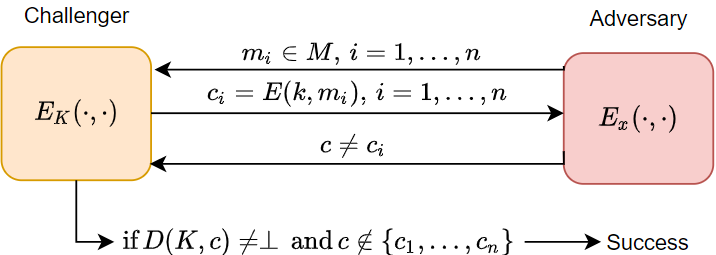
\includegraphics[width=0.8\textwidth]{image/cca.png}
    \caption{CCA Oracle game}
    \label{fig:ciphertextoracle}
\end{figure}
\subsection{Associated Data}
Quando trasmettiamo dei dati c'è spesso la necessità di trasmettere una parte dei dati in chiaro, ad esempio in un pacchetto TCP/IP il cui header può restare in chiaro. Quello che vorremmo però è che l'autenticazione venga fatta \textbf{su tutto} il pacchetto.\\
Possiamo avere due casi limite, tipicamente:
\begin{itemize}
    \item No Associated Data: è sufficiente CCA-Secure Encryption, quindi tutto è cifrato.
    \item No Encrypted Data: è sufficiente un MAC costruito in modo sicuro (\cref{def:hmac}). 
\end{itemize}
Gli algoritmi di AEAD possono lavorare in modo diverso:
\begin{itemize}
    \item Two-Layer: prima cifro e poi applico MAC \textit{(es: AES-GCM)}.  Poiché servono due iterazioni, è un meccanismo più lento e non parallelizzabile poiché per produrre il MAC serve il ciphertext.
    \item One-Layer: faccio cifratura e MAC contemporaneamente \textit{(es: OCB)}. Più veloce \textit{(online cipher)}.
\end{itemize}
\begin{remark}
Le performance sono fondamentali al giorno d'oggi visto che è file sono grandi giga e giga. 
\end{remark}
Ad ogni modo, possiamo osservare due problemi fondamentali:
\begin{problem}[ Dove posizionare la parte di Associated Data?]Tipicamente non c'è una risposta, poiché dipende dal protocollo. Ad esempio se parliamo di header dovrà andare in testa, in altri casi alla fine o anche un mix tra la parte di cifratura e in chiaro. 
\end{problem}
\begin{problem}[ Misuse Resistance]
Quanto è robusto un meccanismo di AEAD quando un IV si ripete?
\end{problem}
\vspace{-5mm}
\section{AES-GCM: Galois Counter Mode}
\vspace{-5mm}
Algoritmo usato nella maggior parte dei protocolli di sicurezza come IPsec e TLS, che usa una struttura \textbf{Enc-than-MAC}. 
\begin{itemize}
    \item \textbf{Encryption:} AES-CTR (\cref{def:ctrmode}).
    \item \textbf{MAC:} GHASH function. Non una crypto-hash ma una struttura algebrica \footnotetext{\href{https://it.wikipedia.org/wiki/Campo_finito}{Galois Field}} per fare prodotti tra polinomi in modo molto veloce. \textbf{Non garantisce sicurezza crittografica}.
\end{itemize}
\begin{definition}[AES-GCM - Galois Counter Mode]\label{def:aesgcm}
Data la chiave $K$, AES-GCM opera nel seguente modo:
\begin{itemize}
    \item \textbf{Key-Derivation:} Poiché la \textbf{chiave} di \textbf{cifratura} \textbf{DEVE} essere \textbf{diversa} \textbf{da} quella di \textbf{autenticazione}, produciamo una chiave $H$, usata per produrre il MAC.
    \item \textbf{AES-CTR:} La parte di cifratura del messaggio viene svolta come in CTR\footnotemark(\cref{def:ctrmode}) \textbf{partendo da 1}, ma ogni ciphertext ottenuto produce un MAC ottenuto tramite il blocco $GM(H)$ per mezzo di prodotti tra polinomi. Il MAC ottenuto va in xor con il ciphertext sucecssivo per produrre un nuovo MAC.
    \item \textbf{Lenght-Check:} Alla fine della cifratura, l'ultimo MAC prodotto viene messo in xor con la lunghezza del ciphertext complessivo per produrre un nuovo MAC. 
    \begin{remark}
    L'aggiunta del controllo sulla lunghezza protegge la costruzione del MAC da un expansion attack.
    \end{remark}
    \item \textbf{Wegman-Carter MAC:} Il MAC della lunghezza viene messo in xor con un keystream ottenuto in CTR-mode ma con contatore $0$ per produrre un MAC \textbf{sicuro}. 
    \begin{remark}
    L'IV usato a questo step sarà \textbf{SEMPRE} diverso in quanto il contatore iniziale era 1. 
    \end{remark}
\end{itemize}
\footnotetext{\textsuperscript{\thefootnote}Il blocco $AES_k$ è una Pseudo-Random Function (PRF).}
\end{definition}
\begin{corollary}[Wegman-Carter Construction]\label{cor:wegmancarter}

Il MAC costruito tramite GCM è una costruzione di tipo Wegman-Carter. Questa costruzione ci fornisce un modo di creare un codice di autenticazione anche quando \textbf{non usiamo} delle funzioni crittografiche. Abbiamo però bisogno di due elementi fondamentali:
\begin{itemize}
    \item Funzioni Hash \textbf{Universali}.
    \item Pseudo Random Functions.
\end{itemize}
\end{corollary}
Le funzioni hash universali sono una famiglia di funzioni dette \textbf{"Key-Hash Function"} il cui output \textbf{dipende} dalla specifica chiave con cui la funzione è inizializzata. In particolare:
\begin{definition}[Universal Hash Functions]
Una famiglia di Key-Hash Function è detta universale se è difficile, per un attaccante che \textbf{non conosce la chiave}, trovare una collisione tale che $H_k(M_1)=H_k(M_2)$.\\
Analogamente: $\forall{x,y}\,:\,x\ne{y}\, Prob\{H_x(M)=H_y(M)\}\leq{1/m}$, con $m$ dimensione del digest. 
\end{definition}
Rispetto ad una crypto hash, le differenze principali stano nel fatto che 
\begin{itemize}
    \item \textbf{se la chiave è nota} trovare una collisione  \textbf{può essere facile}.
    \item L'output \textbf{potrebbe non essere} pseudorandomico.
    \item Dalla seconda proprietà: Un cambio di chiave dovrebbe provocare un cambio nel digest in modo causale e quindi ridurre drasticamente la probabilità di collisione.
    \item Dalla seconda proprietà: Non dovrebbero esserci coppie di messaggi che producono lo stesso hash per chiavi diverse. 
\end{itemize}
\begin{figure}[H]
    \centering
    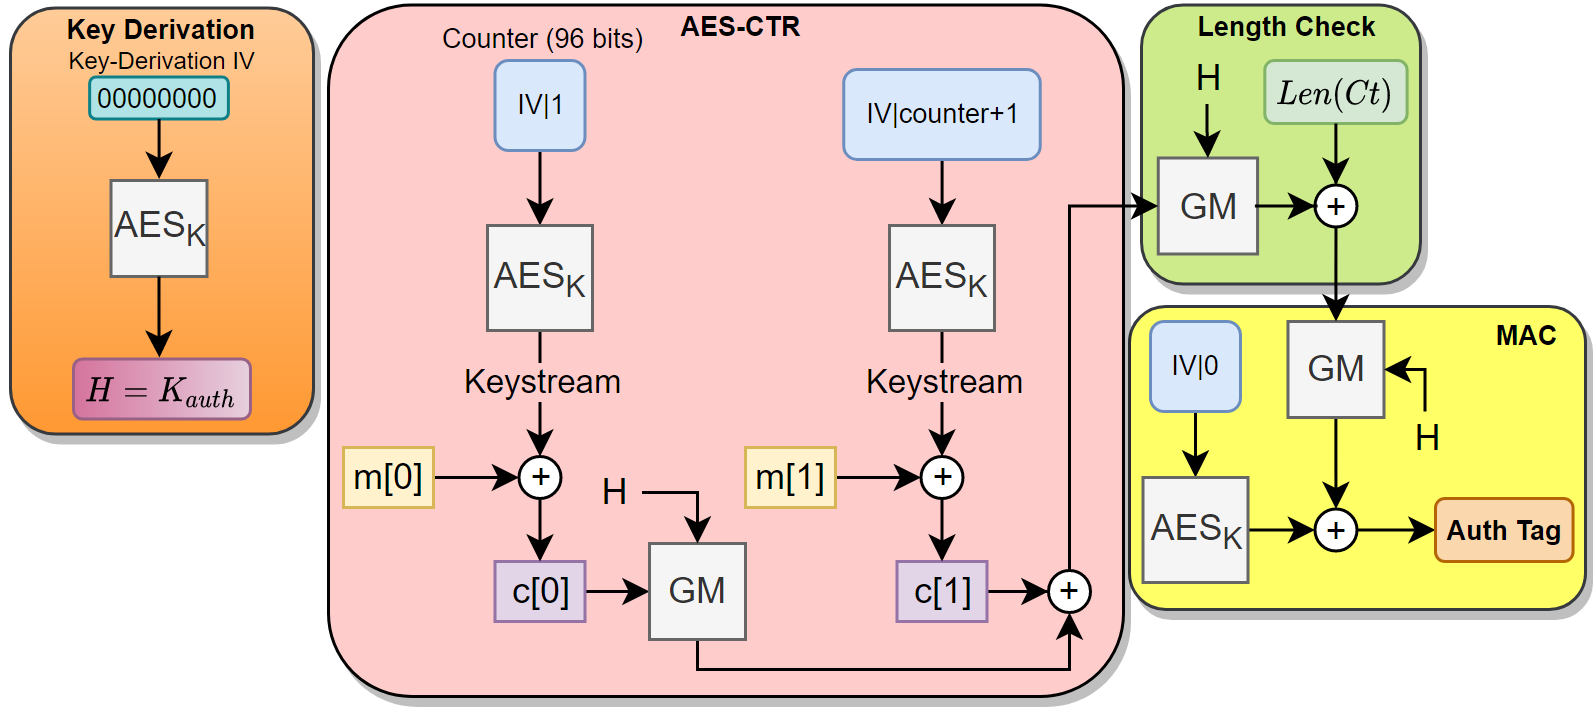
\includegraphics[width=0.8\linewidth]{image/aesgcm.png}
    \caption{AES-GCM scheme}
    \label{fig:aesgcm}
\end{figure}
\begin{remark}\textbf{Come tratto la parte di Dati Associati?}
Semplice: Per ogni blocco di AD produco un MAC che va in xor con il blocco successivo per produrre un nuovo MAC. Alla fine della parte di AD, il MAC va in xor con il primo ciphertext e si continua come indicato in \cref{fig:aesgcm}. La differenza \textbf{sostanziale} sta nell'\textbf{allungare} la dimensione del messaggio complessivo, che ora deve comprendere anche la parte di AD.
\end{remark}

\subsection{Misuse Resistance per GCM}
La costruzione trovata è utile ma ha un problema \textbf{fondamentale:} \textbf{E' LINEARE}, su due aspetti. 
\begin{enumerate}
    \item Il tag è lineare in xor in quanto: $tag=GHASH_H(CT)\oplus{AES_K(IV,0)}$. Pertanto, dati due tag
    \begin{equation*}
        \begin{aligned}
            tag_1&=GHASH_H(CT_1)\oplus{AES_K(IV,0)}\\
            tag_2&=GHASH_H(CT_2)\oplus{AES_K(IV,0)}\\
            tag_1\oplus{tag_2}&=GHASH_H(CT_1)\oplus{GHASH_H(CT_1)}
        \end{aligned}
    \end{equation*}
    \item Poiché la GHASH function usa una moltiplicazione tra polinomi, un attaccante può sempre recupeare la chiave di auth e forgiare dei messaggi validi (\textit{\textbf{la chiave $K$ comunque rimane segreta}}.
\end{enumerate}
Esistono chiaramente delle costruzioni più robuste quando si verifica il riutilizzo di una nonce, ma nnon le trattiamo in questo momento.